% Template for FPL 2012 papers; to be used with:
%          spconf.sty   - ICASSP/ICIP LaTeX style file
%          IEEEtran.bst - IEEE bibliography style file

% Created:  Apr-May 2005 - Riku Uusikartano -- riku.uusikartano@tut.fi
% Modified: March-2012 - Daniel Mu�oz Arboleda -- damuz@unb.br
% --------------------------------------------------------------------------

\documentclass[10pt,a4paper]{article}

\usepackage{spconf,amsmath,epsfig}
\usepackage[brazilian]{babel} % Suporte para o Portugu�s
\usepackage[latin1]{inputenc} % Suporte para acentua��o sem necessidade dos comandos especiais.
\usepackage[]{subfigure}
\usepackage[portuguese,algoruled,longend]{algorithm2e}
\usepackage{multirow}
\usepackage{float}


% Titulo do documento
% -------------------
\title{Projeto de um Rob� Aut�nomo Seguidor de Ectoplasma}


% Nome dos autores
% ----------------
\name{Leonardo Amorim de Ara�jo}
\address{Programa de Gradua��o em Engenharia Eletr�nica, Faculdade Gama\\
Universidade de Bras�lia\\
Gama, DF, Brasil\\
email: leonardoaraujodf@gmail.com}


\hyphenation{Tam-pe-re ela-bo-ra-cao}

\begin{document}

\maketitle

\begin{resumo}
Este documento apresenta como foi realizado o projeto de um rob� aut�nomo seguidor de ectoplasma (subst�ncia flu�dica que os fantasmas deixam aonde passam) cuja fun��o � seguir, encontrar e capturar fantasmas. Este mostra de forma detalhada como foi realizado o projeto e o teste experimental. O microcontrolador utilizado foi o MSP430\cite{davies2008msp430} modelo g2553.
\end{resumo}
\section{Introdu��o}

A an�lise do ectoplasma pode ser realizada de diversos n�veis, seja utilizando dispositivos com hardware program�vel, como FPGAs, ou via software atrav�s de um microcontrolador. A vantagem de se utilizar uma FPGA neste caso � que o rob� ganha muito desempenho e velocidade de processamento, pois o projetista cria um hardware dedicado para a tarefa especificada, utilizando a metodologia das m�quinas de estado ou Projeto RTL\cite{vahid2011digital}, por exemplo. Via de regra, parece ser a solu��o mais interessante, por�m, como j� � da natureza do problema, os sensores possuem sa�da anal�gica, ou seja, fornecem tens�es que variam em uma faixa (0 � 3V, no caso da fam�lia CMOS). Sendo assim, seria necess�rio que a FPGA possu�sse internamente um conversor A/D que pudesse converter os dados anal�gicos atrav�s da amostragem e quantiza��o. Apesar de ser poss�vel, esta tarefa torna o projeto extremamente �rduo de se realizar dentro do tempo requerido, e � nesse aspecto que um microcontrolador faz mais sentido. O microcontrolador MSP430 utilizado neste projeto possui um conversor A/D de 10 bits\cite{davies2008msp430}, que l� valores em uma faixa de 0 � 3V, tendo portanto uma faixa de $3\:V/1024\:\rm{valores} = 3 mV$ em cada passo lido. Esta precis�o grande torna-o �til para a an�lise de dados anal�gicos que possuem varia��o bem pequena de tens�o (que � o caso do ectoplasma dos fantasmas).  

Com os valores obtidos de cada sensor � uma taxa de amostragem relevante para o ataque e destrui��o do fantasma, � poss�vel programar o microcontrolador atrav�s da linguagem C para que este possa setar ou n�o as sa�das e realizar as tarefas especificadas pelo problema, tudo isto dentro do tempo de amostragem do problema. 

O microcontrolador MSP430 j� possui diversas defini��es prontas para serem utilizadas caso seja necess�rio um conversor A/D, um rel�gio (clock) bem exato e al�m disso comuni-ca��o serial (caso, por exemplo, fosse necess�rio saber por GPS onde o rob� se encontra no momento, ou por WIFI).
\section{Experimento}

Para mostrar que � poss�vel realizar a proposta requerida, os sensores de ectoplasma foram simulados utilizando LDRs, que s�o compat�veis pois estes variam sua resist�ncia el�trica conforme a incid�ncia de luz. As sa�das para acionamento dos motores esquerdo, direito e da arma de pr�tons, foram simuladas utilizados LEDS.

\subsection{Fluxograma do Projeto}

Como o projeto foi realizado com um microcontrolador, n�o � relevante usar m�quina de estados pois as a��es n�o s�o realizadas ap�s pulsos de clock, e sim um fluxograma que apresenta as a��es tomadas.

\subsection{Convers�o Anal�gico-Digital}

A figura \ref{fig1} apresenta como foi realizada a convers�o anal�gico-digital usando o MSP. No c�digo apresentado na refer�ncia, as fun��es \textit{Setup\_ADC} e \textit{Read\_ADC()} tem o objetivo de realizar a configura��o inicial do Conversor A/D e a leitura dos valores anal�gicos nos pinos P1.0, P1.1, P1.2 e P1.3, respectivamente. Os valores convertidos ser�o armazenados nas vari�veis \textit{ADC[0]}, \textit{ADC[1]}, \textit{ADC[2]} e \textit{ADC[3]}. Posteriormente, na fun��o \textit{Ler\_Sensores()}, os valores destas vari�veis ser�o atualizadas para que os dados obtidos de tens�o sejam tratados, de forma que ser�o atribu�dos os valores lidos �s vari�veis:
 
\begin{itemize}
	\item \textit{SENSOR\_FRONTAL = ADC[3]}
	\item \textit{SENSOR\_TRASEIRO = ADC[2]}
	\item \textit{SENSOR\_ESQUERDO = ADC[1]}
	\item \textit{SENSOR\_DIREITO = ADC[0]}
\end{itemize}

\begin{figure}[htbp]
	\centering
	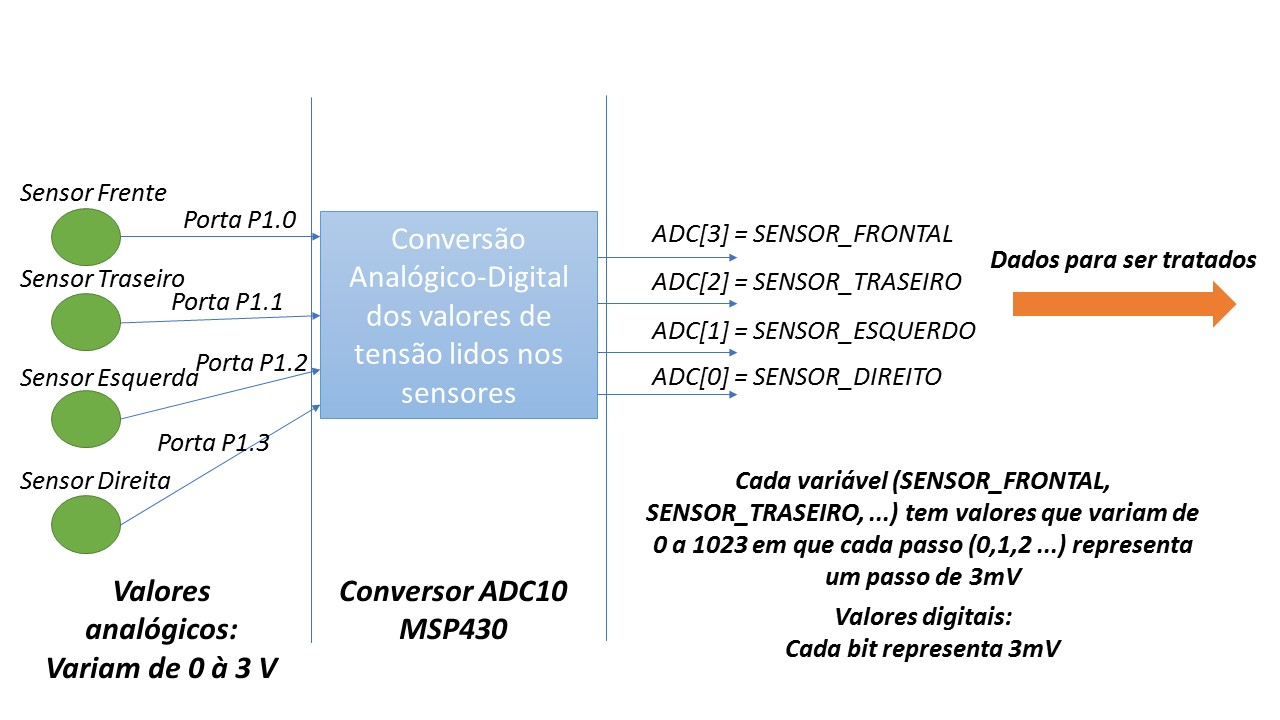
\includegraphics[scale=0.25]{Figura1.jpg}
	%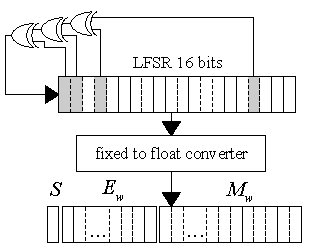
\includegraphics[scale=0.9]{figures/fig1_RNG.eps}
	\caption{Fluxograma mostrando como foi realizado a convers�o anal�gico-digital}
	\label{fig1}
\end{figure}

\subsection{A��es a serem realizadas ap�s a convers�o}

A figura \ref{fig2} apresenta o fluxograma das a��es tomadas pelo microcontrolador ap�s a convers�o anal�gico-digital ser realizada. Na fun��o \textit{Ler\_Sensores()}, todas estas a��es s�o realizadas. � importante destacar que as sa�das est�o declaradas nas seguintes portas do microcontrolador:

\begin{itemize}
	\item P1.4 - MOTOR ESQUERDO
	\item P1.5 - MOTOR DIREITO
	\item P1.6 - ARMA
\end{itemize}

onde o valor l�gico 1 representa acionamento e valor l�gico 0, desligamento. A fun��o \textit{Ler\_Sensores()} segue o seguinte procedimento:

\begin{itemize}
	\item Caso a m�dia dos valores dos sensores lidos seja menor que 20, ou seja, menor que 20*3 mV = 60 mV, isto quer dizer que a queda de tens�o nos LDRs foi grande, significando que a incid�ncia de luz est� alta sobre os sensores, e em todos ao mesmo tempo. Desta forma, � poss�vel que um fantasma esteja muito pr�ximo do rob� e deve-se atacar. Chama-se a fun��o \textit{Selecao\_Saida()} que seleciona qual sa�da ser� acionada. Nesta hora, o rob� parar�, a arma ser� acionada, ser� esperado 1 segundo para o disparo, e mais 9 segundos para que a arma de pr�tons possa estabilizar, conforme requerido pela proposta de projeto. Ap�s isto, ser� realizado mais uma leitura dos sensores, e ser� verificado se ainda h� exist�ncia do fantasma, realizando o mesmo procedimento em loop descrito.
	\item Caso o valor do sensor frontal seja maior que a m�dia dos valores dos sensores lidos mais um par�metro de m�dia, que � definido pelo projetista (por exemplo, existem ectoplasmas que s�o dif�ceis de se detectar, ent�o o par�metro de m�dia deve ser baixo, j� para outros fantasmas, aumenta-se o valor desta constante) o rob� deve seguir em frente, pois o sensor frontal detecta ectoplasma � certa dist�ncia.
	\item Caso o valor do sensor esquerdo seja maior que a m�dia dos valores dos sensores lidos mais o par�metro de m�dia, o rob� deve virar a esquerda, desligando o motor da direita.
	\item Caso o valor dos sensores direito ou traseiro sejam maiores que m�dia dos valores lidos mais o par�metro de m�dia, o rob� deve virar � direita, desligando o motor da esquerda. Veja que, quando o sensor traseiro estiver acionado, j� que o rob� n�o pode mover para tr�s, � necess�rio que este gire 180�, virando � direita totalmente, e assim o sensor frontal ser� acionado, e desta forma, este seguir� em frente. Neste ponto, pode existir uma falha, pois o fantasma se for r�pido, pode enganar o rob�, devendo-se posteriormente criar uma arma que seja utilizada com servo-motores, por exemplo.
	\item Se nenhum sensor for acionado, ou seja, n�o existir presen�a de ectoplasma, o rob� ir� seguir reto. Os projetistas podem posteriormente mudar esta condi��o.
\end{itemize}

	Em cada caso, ap�s o acionamento dos motores, espera-se 100 ms para se realizar uma nova convers�o. Isto � interessante para estabilidade do motor, pois ele pode come�ar a tremer muito, caso os valores mudem com rapidez (no caso do acionamento da arma, espera-se 10 segundos, utilizado a fun��o \textit{Atraso()} que utiliza o TimerA do MSP430).
	
\begin{figure}[htbp]
	\centering
	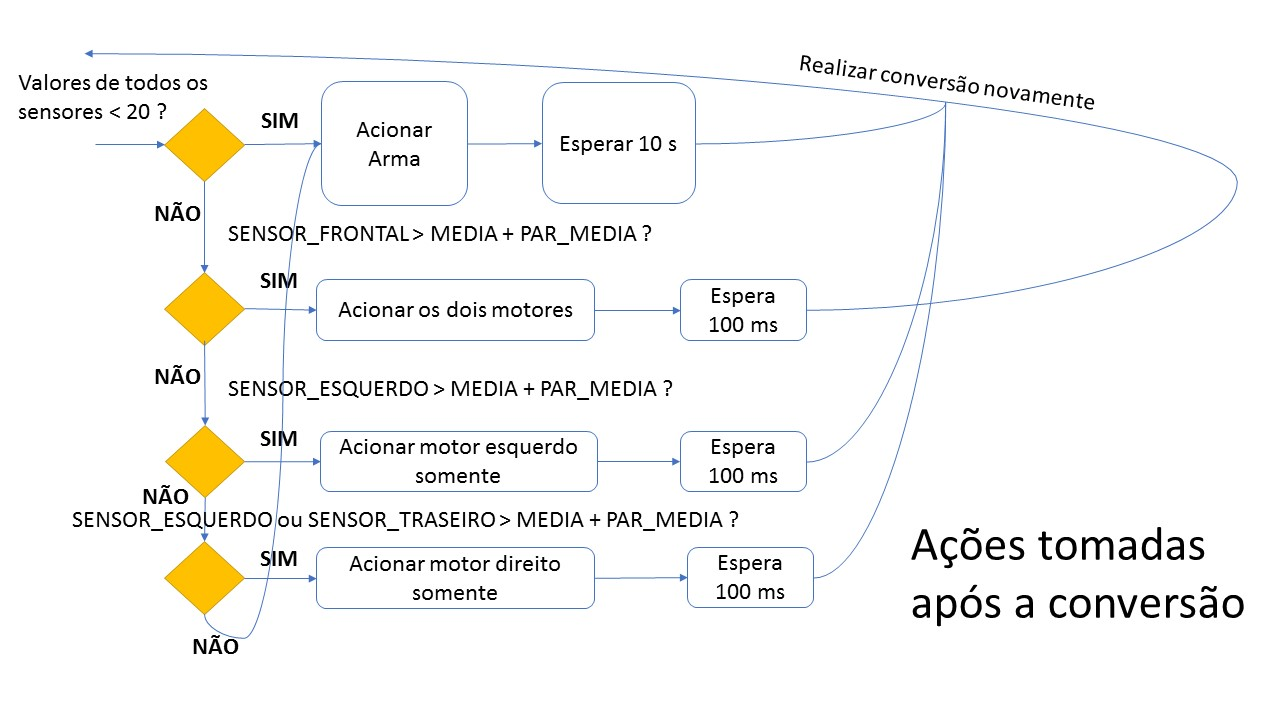
\includegraphics[scale=0.25]{Figura2.jpg}
	%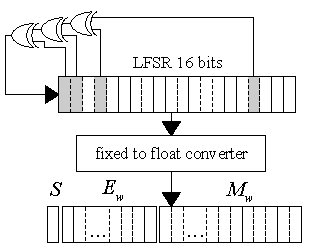
\includegraphics[scale=0.9]{figures/fig1_RNG.eps}
	\caption{Fluxograma mostrando as a��es tomadas ap�s a convers�o}
	\label{fig2}
\end{figure}

\subsection{Material Utilizado}

A tabela \ref{Materiais_utilizados} apresenta todos os dispositivos e componentes utilizados no projeto.

\begin{table}[!h]\centering
	\caption{Materiais Utilizados no Experimento}
	\label{Materiais_utilizados}
	\begin{tabular}{c p{5 cm}}\centering
		Quantidade & Material \\
		\hline
		4 & Resistores de de $10,00 \pm 0,50$ k$\Omega $ (1/4 W)\\
		3 & Resistores de $1,00 \pm 0,05$ k$\Omega $ (1/4 W) \\ 
		4 & Resistores Dependentes de Luz - LDRs \\
		1 & Mini-Protoboard\\
		3 & LEDs\\			
		1 & Microcontrolador MSP 430 modelo G2553 \\

		\hline				
	\end{tabular}
\end{table}


\section{Resultados}

Como nesta simula��o foram utilizados LDRs, a luz ambiente interfere na varia��o de tens�o do resistores. Logo em cada resistor, foi colocado um peda�o de fita isolante para que estes se comportem como se estivessem "na escurid�o", e a tens�o que ser� lida ser� pr�xima do m�ximo, ou seja, 3V.
A figura \ref{fig3} apresenta a simula��o utilizando LEDs para representar os motores e a arma. Neste caso, quando o LDR que representa o sensor esquerdo, que fica na porta P1.2 ficou sem a fita isolante, o motor esquerdo foi acionado (LED Aceso), ou seja, a sa�da P1.4 foi acionada no MSP. Al�m disso, veja que, os dois outros LEDS ficaram desligados, e estes representam a arma e o motor direito.
J� na figura \ref{fig4}, pode-se visualizar que ao deixar o LDR que representa o sensor direito (ligado � porta P1.3) ficou sem fita isolante, e desta forma o motor direito foi acionado (porta P1.5), e o os outros dois LEDs ficaram desligados. Da mesma forma, quando o sensor traseiro (ligado � porta P1.1) ficou sem fita isolante, somente este LED ficou aceso.
Na figura \ref{fig5}, pode-se visualizar que quando o LDR que representa o sensor frontal foi acionado (porta P1.0), os LEDs que representam os dois motores foram acionados (Portas P1.4 e P1.5).
E por fim, na figura \ref{fig6}, pode-se visualizar que, quando todos os LDRs est�o sem fita isolante, o que representa que todos os sensores est�o acionados, o LED que representa a arma dispara. Pode-se verificar tamb�m que o tempo de acionamento foi realmente de 1 segundo, e o MSP esperou 10 segundos para realizar outro disparo (acionou o led).

\begin{figure}[H]
	\centering
	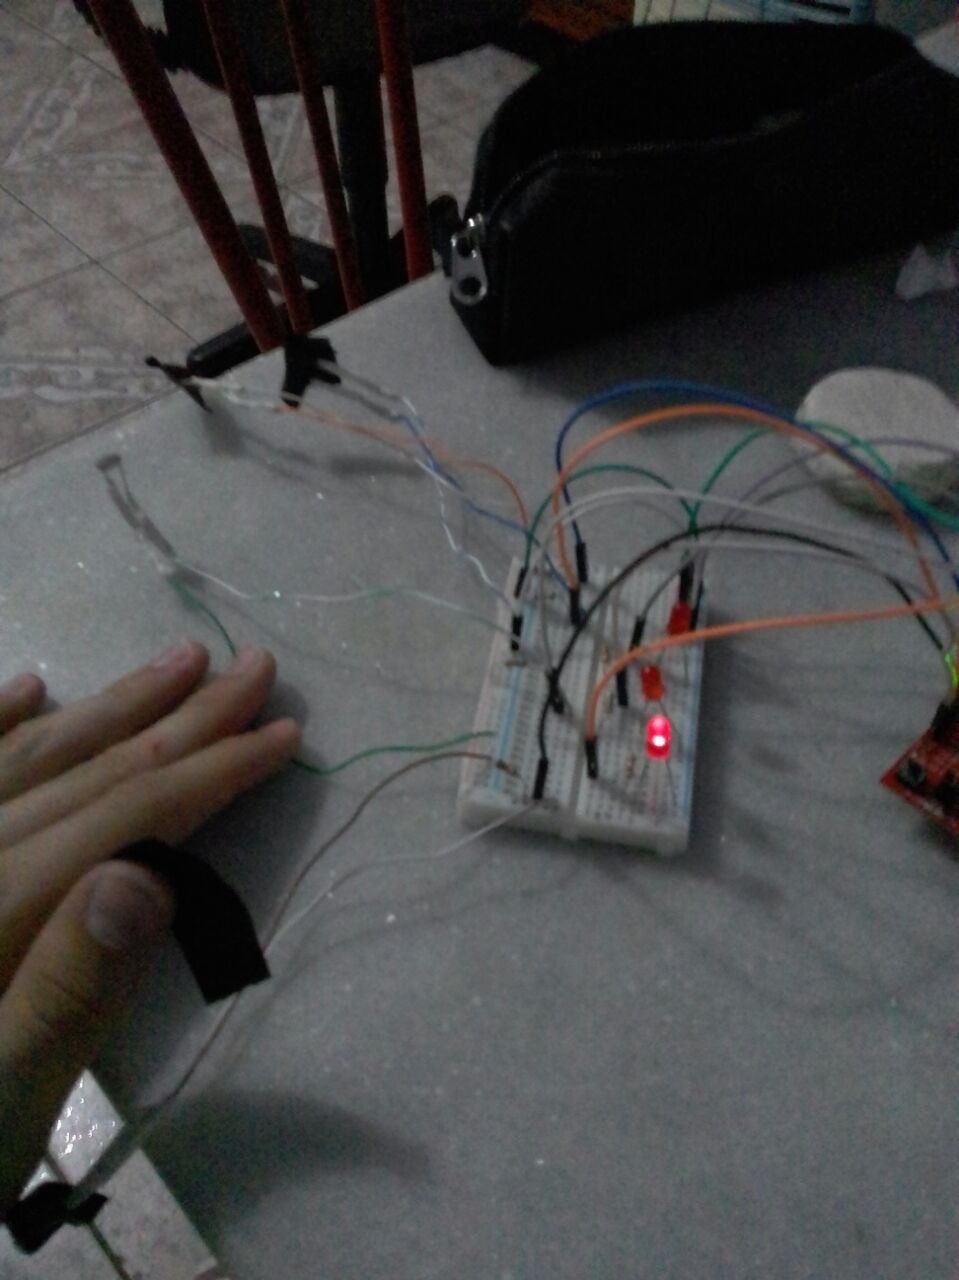
\includegraphics[scale=0.10]{resultado1.jpeg}
	%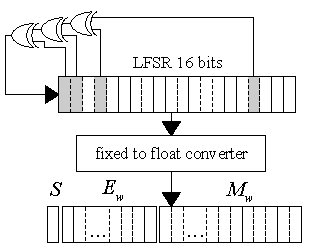
\includegraphics[scale=0.9]{figures/fig1_RNG.eps}
	\caption{Sensor Esquerdo sem fita-isolante, motor direito acionado - Representa��o com LEDs}
	\label{fig3}
\end{figure}


\begin{figure}[H]
	\centering
	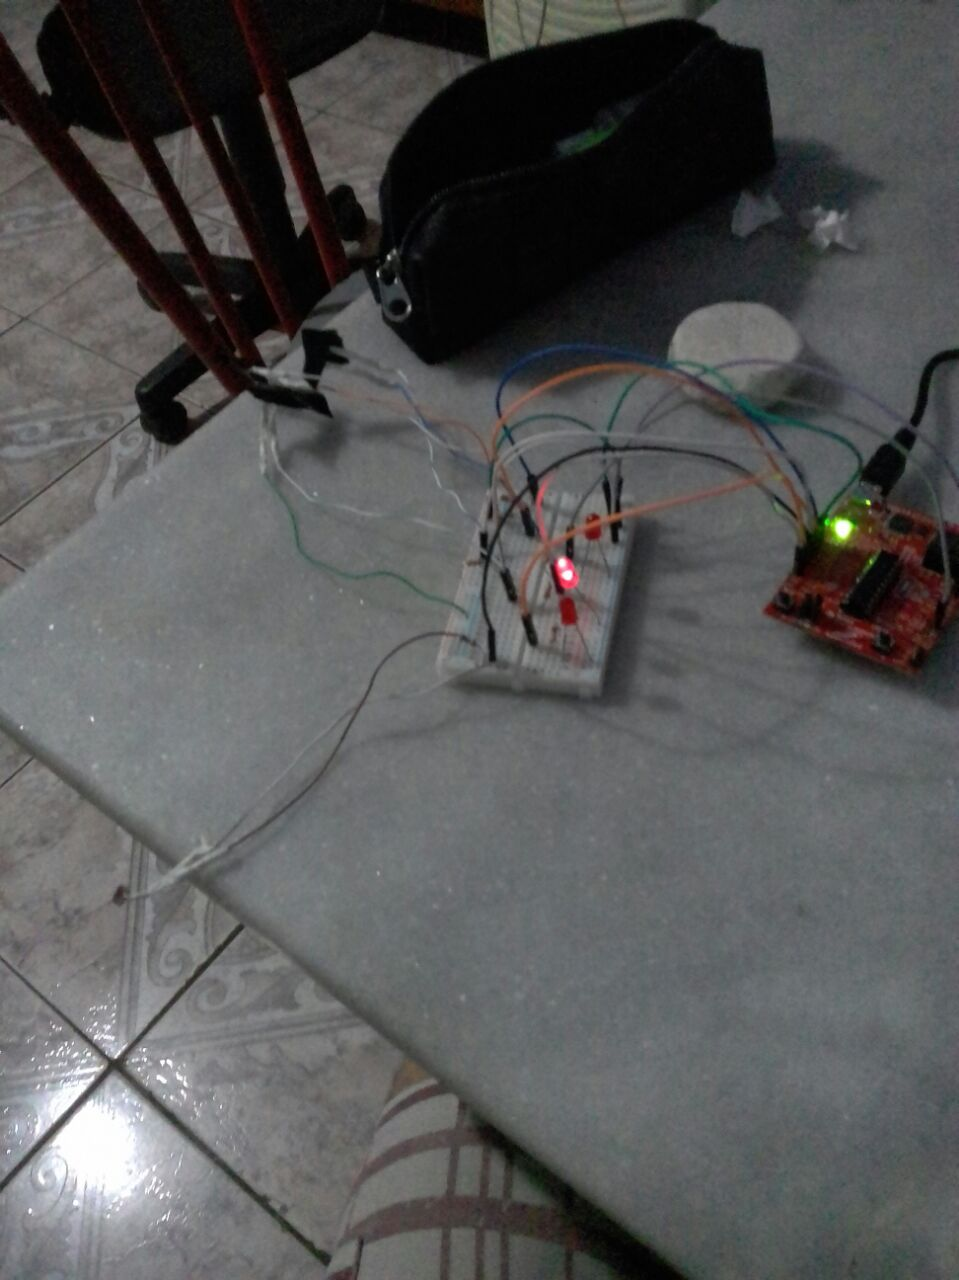
\includegraphics[scale=0.10]{resultado2.jpeg}
	%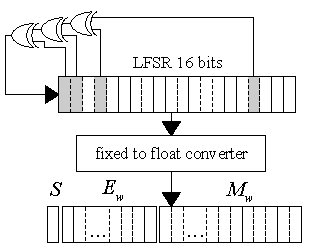
\includegraphics[scale=0.9]{figures/fig1_RNG.eps}
	\caption{Sensor Direito sem fita-isolante, motor direito acionado. O mesmo ocorre se o sensor traseiro � acionado (fica sem fita isolante) - Representa��o com LEDs}
	\label{fig4}
\end{figure}


\begin{figure}[H]
	\centering
	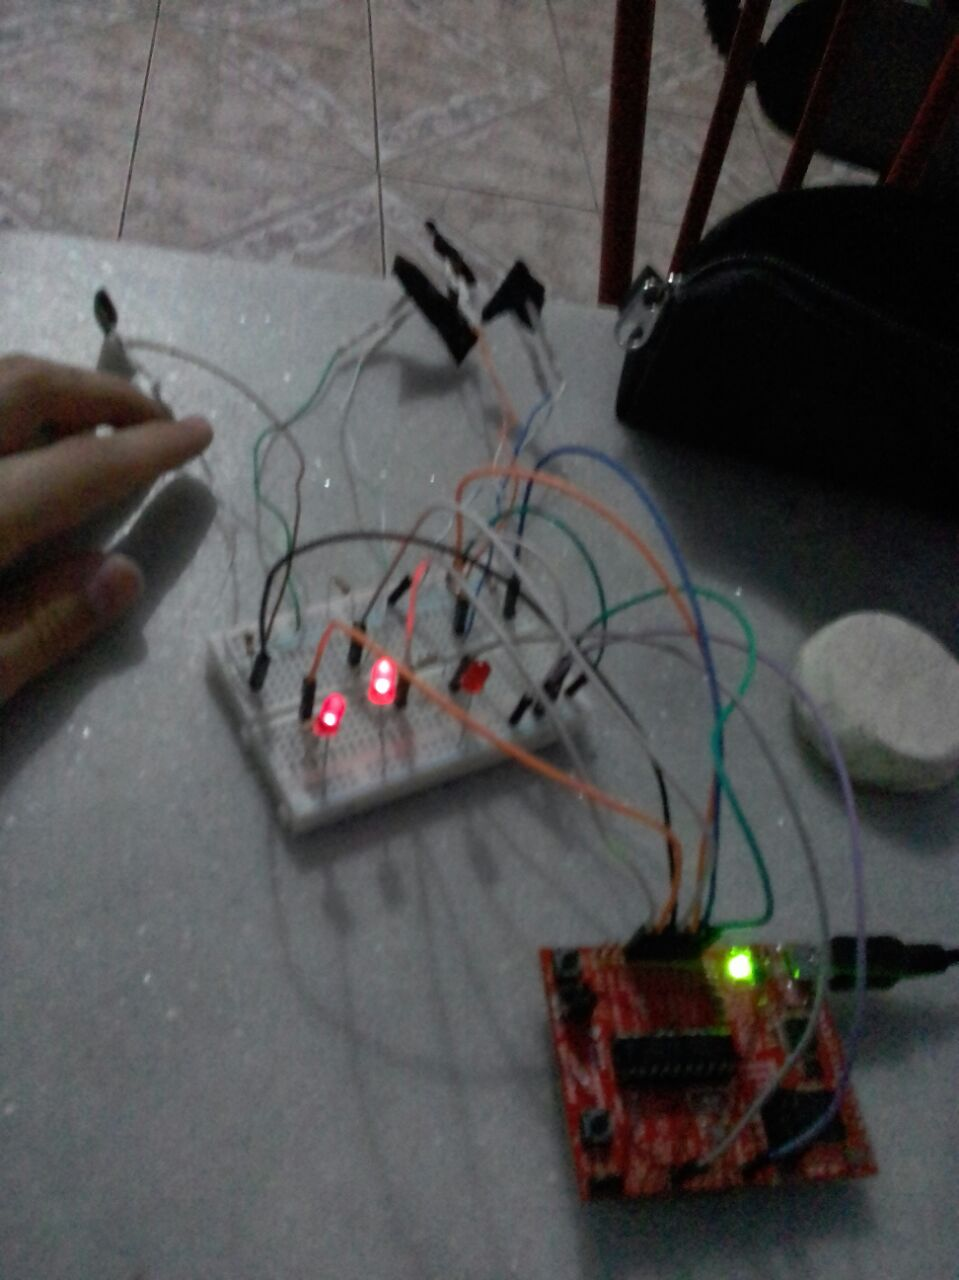
\includegraphics[scale=0.10]{resultado3.jpeg}
	%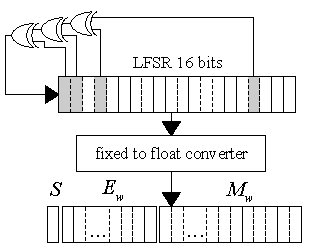
\includegraphics[scale=0.9]{figures/fig1_RNG.eps}
	\caption{Sensor Frente sem fita-isolante, motor direito e esquerdo acionado - Representa��o com LEDs}
	\label{fig5}
\end{figure}

\begin{figure}[H]
	\centering
	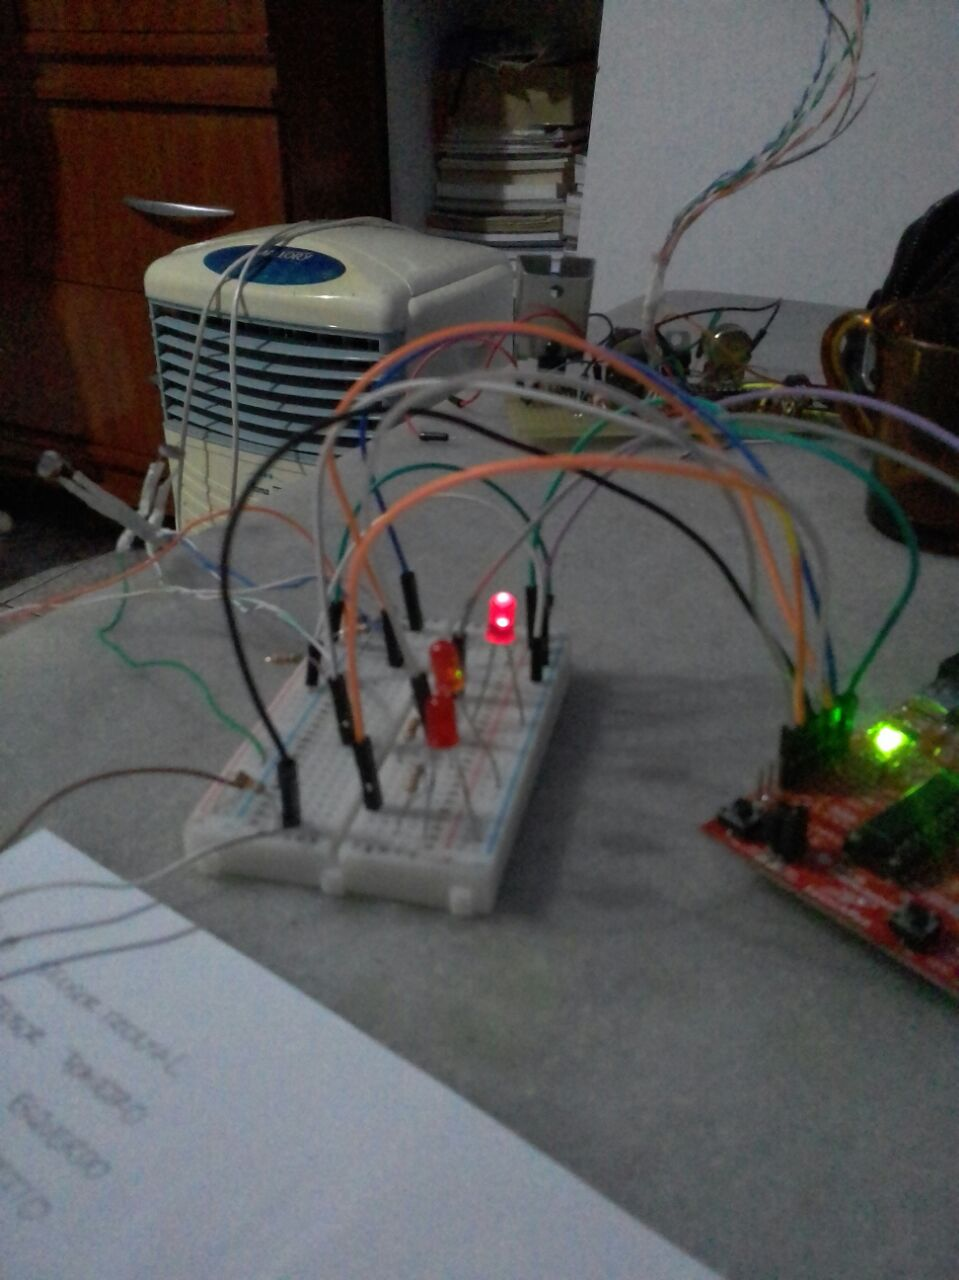
\includegraphics[scale=0.10]{resultado4.jpeg}
	%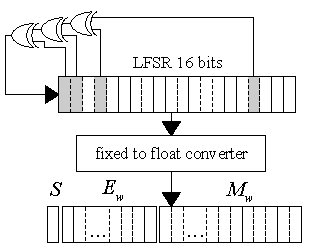
\includegraphics[scale=0.9]{figures/fig1_RNG.eps}
	\caption{Todos os Sensores Acionados, Arma disparada - Representa��o com LEDs}
	\label{fig6}
\end{figure}
\section{Discuss�o e Conclus�es}
Conclui-se portanto que nesta proposta, � poss�vel realizar o projeto do rob� atrav�s do microcontrolador MSP430 e que este consegue com facilidade atender aos requisitos da proposta em quest�o, conseguindo inclusive, incorporar mais prot�tipos, como um m�dulo GPS ou WIFI para descobrir a localiza��o do rob�.
Verificou-se que, com os LDRs utilizados como sensores, os motores e a arma foram acionadas praticamente com precis�o. Apesar disto, algumas pontos interessantes podem ser melhorados, como o fato de que o rob� pode se mover pra frente e para tr�s, evitando  que este tenha que girar 180� para acompanhar um fantasma que aciona o sensor traseiro. O projeto com microcontrolador pode ser interessante para um futuro prot�tipo utilizando FPGAs, pois pode-se utilizar a mesma l�gica para cria��o de um hardware\cite{vahid2011digital} que realiza as tarefas que o MSP realiza.
Um outro aspecto interessante seria considerar uma arma m�vel, que girasse num eixo (que poderia ser feito com servomotores), para que esta ficasse exatamente na dire��o do fantasma na hora do tiro.
\section{Anexos}
\subsection{C�digos}

Todos os c�digos utilizados podem ser verificados no github a seguir: 

\small
% IEEEtran is a LaTeX style file defining the reference formatting.
% -----------------------------------------------------------------
\bibliographystyle{IEEEtran}
\bibliography{IEEEabrv,labrefs}
%\bibliography{IEEEabrv,fpl_refs}


\end{document}